%% ****** Start of file aiptemplate.tex ****** %
%%
%%   This file is part of the files in the distribution of AIP substyles for REVTeX4.
%%   Version 4.1 of 9 October 2009.
%%
%
% This is a template for producing documents for use with 
% the REVTEX 4.1 document class and the AIP substyles.
% 
% Copy this file to another name and then work on that file.
% That way, you always have this original template file to use.

%\documentclass[aip,graphicx]{revtex4-1}
%\documentclass[aip,reprint]{revtex4-1}

%\usepackage{graphicx}

%\draft % marks overfull lines with a black rule on the right
\documentclass[pre,aps,floatfix,authordate1-4,twocolumn]{revtex4-1}
%\documentclass[pre,aps,floatfix,authordate1-4]{revtex4-1}

%\documentclass[aps,prl,preprint,superscriptaddress]{revtex4}



%\documentclass[aps,prl,preprint,groupedaddress]{revtex4}

\usepackage{rotating} 
\usepackage{times}
\usepackage{graphicx}
\usepackage{setspace}
\usepackage{amsmath}
\usepackage{epstopdf}
\usepackage[obeyFinal]{easy-todo}
\begin{document}

% Use the \preprint command to place your local institutional report number 
% on the title page in preprint mode.
% Multiple \preprint commands are allowed.
%\preprint{}

\title{Rotational dynamics of proteins from spin relaxation times and molecular dynamics simulations} %Title of paper

% repeat the \author .. \affiliation  etc. as needed
% \email, \thanks, \homepage, \altaffiliation all apply to the current author.
% Explanatory text should go in the []'s, 
% actual e-mail address or url should go in the {}'s for \email and \homepage.
% Please use the appropriate macro for the type of information

% \affiliation command applies to all authors since the last \affiliation command. 
% The \affiliation command should follow the other information.

\author{O. H. Samuli Ollila}
\email[]{samuli.ollila@helsinki.fi}
%\homepage[]{Your web page}
%\thanks{}
\affiliation{Insititute of Biotechnology, University of Helsinki}
\affiliation{Institute of Organic Chemistry and Biochemistry,
Czech Academy of Sciences, 
Prague 6, Czech Republic}

\author{Hideo Iwai}
%\homepage[]{Your web page}
%\thanks{}
\affiliation{Insititute of Biotechnology, University of Helsinki}

% Collaboration name, if desired (requires use of superscriptaddress option in \documentclass). 
% \noaffiliation is required (may also be used with the \author command).
%\collaboration{}
%\noaffiliation

\date{\today}

\begin{abstract}
  % insert abstract here
  
\end{abstract}

%\pacs{}% insert suggested PACS numbers in braces on next line

\maketitle %\maketitle must follow title, authors, abstract and \pacs

% Body of paper goes here. Use proper sectioning commands. 
% References should be done using the \cite, \ref, and \label commands


%\label{}
\section{Introduction}
Conformational sampling and entropy of proteins
play a significant role in functionality
and interactions with other biomolecules.
In addition to internal dynamics due to conformation sampling, the
proteins also experience overall brownian tumbling.
These properties are experimentally accessible through 
spin relaxation times of $^{15}$N and $^{13}$C nucleai measured
with nuclaer magnetic resonance (NMR) 
techniques \cite{jarymowycz06,korzhnev01,bedem15,lewandowski15,lamley15}. 
Spin relaxation rate experiments have been used to, for example, analyze
conformational entropies \cite{kasinath13,allner15,jarymowycz06}, binding entropies \cite{akke93,jarymowycz06},
resolve sampled structures \cite{bedem15}
and validate molecular dynamics simulations \cite{best04,showalter07a,showalter07b,maragakis08,trbovic08}.
These analyzes are almost exclusively based on the
separation of internal conformational sampling 
and overall rotational tumbling \cite{wennerstrom79,Lipari82} and
isotropic overall diffusion is often assumed, while
analysis of anisotropic molecules is significantly more
complicated \cite{jarymowycz06,korzhnev01,luginbuhl97,hall04}.
Thus, new approaches are needed to intepret spin relaxation times
measured from anisotropic or intrinsically disordered molecules.


%This approach has been successfully applied for large amount of proteins
%with isotropic shape and overall rotational diffusion \cite{jarymowycz06}.
%The resulting order parameters and overall rotational diffusion coefficients
%
%, however, proteins
%with anisotropic shape or large amount of internal motional timescales
%are 
%proteins parameter space for fitted parameters become
%rotational diffusion and internal flexibility of proteins and other biomolecules.
%On the other hand, segmental level information has been used in validation
%and improvement of molecular dynamics simulation force fields \cite{??}.
%Segmental order has been also related to conformational entropy of proteins \cite{??}.

 
Classical molecular dynamics simulation methods are
promising tools to interpretate spin relaxation time experiments
for molecules with significant anisotropy or correlations between
internal and overall rotational motions. Practical applications
are, however, limited by inaccuracies in the force field descriptions
and available time scales in the simulations \cite{prompers02,maragakis08,trbovic08,wong08,anderson12}.
The overestimation of overall rotational diffusion due to inaccuracies in 
water models~\cite{wong08} and very long simulations required to calculate rotational
correlation functions with sufficient accuracy from single molecules in MD
simulations \cite{lu06,anderson12} have been the main complications.

In this work we overcome these issues by assuming that the overall
rotational dynamics of protein follows
anisotropic rigid body diffusion around inertia axes. 
Diffusion coefficients are directly calculated from angular displacements of
protein intertia axes and used to determine overall rotation part
of backbone N-H bonds correlation functions.
This reduces the simulation length required for accurate determination
of rotational correlation functions. Furthermore, the overestimated
rotational diffusion due to water model can be anisotropically corrected
by scaling the diffusion coefficients in all directions with a constant
factor. The approach is demonstrated by interpreting the experimental
spin relaxation times of HpTonB-92 \cite{ciragan16} and PsTonB \cite{??}
protein constructs, both having significantly anisotropic shape. 
These protein segments are critical for iron transport into Helicbacteri
Pyroli and Pseudomonas bacteria, respectively.


\section{Methods}

\subsection{Spin relaxation experiments and rotational dynamics of molecules}
Molecular dynamics of protein backbone residues and spin relaxation experiments can
be connected by using the spectral density $J(\omega)$ 
\begin{equation}\label{SPECTdens}
  J(\omega)=2\int_0^\infty C(t) \cos(\omega t) {\rm d}t,
\end{equation}
which is the Fourier transformation of the second order
rotational correlation function for N-H bond vector
\begin{equation}\label{CORRFdef}
  C(t)=\langle \frac{3}{2}\cos^2\theta_{t'+t}-\frac{1}{2} \rangle_{t'},
\end{equation}
where $\theta_{t'+t}$ is the N-H bond angle between times $t'$ and $t'+t$
and angular brackets refer to the ensemble average.
Connection to experimentally measured spin relaxation times $T_1$, $T_2$
and $T_{\rm NOE}$ is given by Redfield equations \cite{abragam,kay89}
\begin{equation}\label{R1}
  \begin{aligned}
  \frac{1}{T_1}= & \frac{d_{\rm{NH}}^2N_{\rm{H}}}{20}\bigg[J(\omega_{\rm{H}}-\omega_{\rm{N}})+3J(\omega_{\rm{N}})+6J(\omega_{\rm{N}}+\omega_{\rm{H}})\bigg] \\
        & +\frac{(\sigma \omega_{\rm{N}})^2}{15}j(\omega_{\rm{N}}),
  \end{aligned}
\end{equation}
\begin{equation}\label{R2}
    \begin{aligned}
  \frac{1}{T_2}= & \frac{1}{2}\frac{d_{\rm{NH}}^2N_{\rm{H}}}{20}\bigg[4J(0)+3j(\omega_{\rm{N}})+J(\omega_{\rm{H}}-\omega_{\rm{N}})+6J(\omega_{\rm{H}})  \\
    & +6J(\omega_{\rm{N}}+\omega_{\rm{H}})\bigg]+\frac{(\sigma \omega_{\rm{N}})^2}{90}[4J(0) +3J(\omega_{\rm{N}})],
    \end{aligned}
\end{equation}
\begin{equation}\label{NOE}
  \frac{1}{T_{\rm NOE}}=1+\frac{d_{\rm{NH}}^2N_{\rm{H}}}{20}\bigg[6J(\omega_{\rm{N}}+\omega_{\rm{H}})+J(\omega_{\rm{H}}-\omega_{\rm{N}}))\bigg]\frac{\gamma_{\rm{H}}}{\gamma_{\rm{N}}R_1},
\end{equation}
where $\omega_{\rm{N}}$ and $\omega_{\rm{H}}$ are the Larmor angular
frequencies of $^{15}$N and $^1$H respectively, and
$N_{\rm{H}}$ is the number of bound protons.
The dipolar coupling constant is given by
\begin{equation}
d_{\rm{NH}}=-\frac{\mu_0\hbar\gamma_{\rm{H}}\gamma_{\rm{N}}}{4\pi\langle r_{\rm{CN}}^3\rangle},\nonumber
\end{equation}
where $\mu_0$ is the magnetic constant or vacuum permeability, $\hbar$ is the reduced Planck constant,
$\gamma_{\rm{N}}$ and $\gamma_{\rm{H}}$ are the gyromagnetic constants of $^{15}$N and $^1$H, respectively.
Average cubic length is calculated as $\langle r_{\rm{CN}}^3\rangle = (0.101{\rm nm})^3$ and the 
value of $\Delta \sigma = -160$ ppm is used for the chemical shift anisotropy of N-H bonds in 
proteins \cite{kay89,hiyama88}.
%Same equations can be used, for example, to C-H bond by changing the
%constants related to nitrogen to the ones corresponding carbon. 

Spin relaxation experiments are typically interpreted by
dividing the rotational dynamics in overall tumbling 
and internal relaxation due to conformational sampling 
and assuming that the motions are 
independent \cite{wennerstrom79,Lipari82,jarymowycz06,korzhnev01}.
The rotational correlation function for chemical bonds can be then written as
\begin{equation}\label{CORRFsep}
  C(t)=C_I(t)C_O(t),
\end{equation}
where $C_I(t)$ and $C_O(t)$ are correlation functions for internal and overall
rotations, respectively. Conformational sampling can be described
in this approximation by using the square of order parameter respect to 
molecular axes $S^2$, which is given by the plateau of the internal rotational 
correlation function, and the effective correlation time 
\begin{equation}
  \tau_{\rm eff}=\int_0^\infty C_I'(t) \mathrm{d}t,
\end{equation}
where $C_I'(t)=\frac{C_I-S^2}{1-S^2}$ is the reduced correlation function \cite{Lipari82}.

The overall rotational correlation function is often described
by approximating protein as a rigid body, which gives 
a sum of five exponentials for fully anisotropic molecule \cite{woessner62,korzhnev01}
\begin{equation}\label{CORRFanisot}
  C_O(t)=\sum_{j=1}^5 A_j e^{-t/\tau_j},
\end{equation}
where time constants $\tau_j$ are related 
to the diffusion constants around
three principal axes of a molecule
($D_{xx}$, $D_{yy}$ and $D_{zz}$)  
\footnote{
$\tau_1=(4D_{xx}+D_{yy}+D_{zz})^{-1}$,
$\tau_2=(D_{xx}+4D_{yy}+D_{zz})^{-1}$,
$\tau_3=(D_{xx}+D_{yy}+4D_{zz})^{-1}$,
$\tau_4=[6(D+(D^2-L^2)^{-1/2}]^{-1}$,
$\tau_5=[6(D-(D^2-L^2)^{-1/2}]^{-1}$,
$D=\frac{1}{3}(D_{xx}+D_{yy}+D_{zz})$ and 
$L^2=\frac{1}{3}(D_{xx}D_{yy}+D_{xx}D_{zz}+D_{yy}D_{zz})$}
and prefactors $A_j$ to the directions of chemical bonds 
respect to the molecular axes \cite{woessner62,luginbuhl97}.

The simplest approach to extract molecular dynamics from experimental
data is the original ''model free analysis'', where monoexponential
decay with time constant $\tau_{\rm eff}$ is assumed for internal correlation
function and isotropic diffusion for overall rotational correlation function \cite{??}.
Equation \ref{CORRFanisot} is monoexponential for isotropic diffusion
and the overall dynamics of such protein can described with single time constant $\tau_c$.
Dynamics for each residue can be described with internal rotational relaxation 
time $\tau_{\rm eff}$ and the order parameter $S^2$. For this simple model
the parameters can be successfully fitted to the experimental data,
however the fitting becomes significantly more difficult for proteins 
with anisotropic overall diffusion or several internal timescales \cite{dosset00,luginbuhl97}.


%Standard analyses of experimental relaxation data usually assume
%fully or axially isotropic overall rotational motion and single
%decay constant for interal motion. Then the free parameters
%($S^2$, $\tau_j$, $A_j$) are fit against spin relaxation data
%from experiments. This gives most likely very good results for
%isotropic molecules for which the assumption of single internal
%motional timescale is reasonable. However, for molecules with
%significant shape anisotropy or several timescales in internal
%motions the amoount parameters to be fitted becomes large compared
%with the typical amount of experimental points.

The 
Two different approaches have been commonly used to analyze
rotational dynamics from NMR relaxation experiments. In
''model free analysis'' the fundamental idea is to separate
interal dynamics from global rotation and assume exponential
forms for rotational correlation functions. The parameters of
rotational correlation functions are then fitted the experimental
data to solve time scales and order parameters for different dynamical
processes \cite{dosset00,??}. Alternative approach is to use bead models and hydrodynamical
calculations to describe protein dynamics and predict spin relaxation rates \cite{torre00}.
The approaches have been successfull or several proteins, but both suffer
from significant limitations which limit the general applicability \cite{??}.
Main practical issue in the ''model free analysis'' is that the amount of
freen parameters to be fitted in the experiments becomes large for anitoropic
proteins experiencing complex dynamics \cite{??}. On the other hand,
hydrodynamical calculations are sentitive for the assumptions about
protein hydration shell \cite{torre00}.


Spin relaxation data is usually analyzed by describing the sampled bond
orientations with order parameter $S^2$ respect to the protein reference frame
and assuming that overall and internal motions are independt \cite{??,korzhnev01}.
Order parameters and timescales for overall and internal motions can be then
extracted by fitting various functional forms to spin relaxation data
measured with different magnetic field strengths \cite{jarymowycz06,korzhnev01}.

%\begin{equation}
%  C'_I(t)= e^{-t/\tau_c},
%\end{equation}


\subsection{Rotational dynamics from molecular dynamics simulations}\label{MDanalysis}
Classical molecular dynamics simulation gives a trajectory for each atom in
a system as a function of time. These trajectories can be used to
calculate rotational correlation functions for each bond from Eq. \ref{CORRFdef}.
The rotational correlation functions can be further used to calculate the
spin relaxation times through Eqs. \ref{R1}-\ref{SPECTdens} and the resulting
values can be compared to experimental data in order to assess simulation model
quality \cite{??} and interpret experiments \cite{??}.
However, the comparison is often complicated by
the short simulation times \cite{??} and incorrect overall rotational
diffusion due to water models \cite{??}.

Here we use overall rotational diffusion constants
calculated from Eq. \ref{DIFFdef} to determine 
the timescales of global rotational correlation function
in Eq. \ref{CORRFanisot}. The rotational
diffusion coefficients are given by a linear fit
to the mean square angle deviation of intertia axes calculated from
simulations (see results and discussion).
Straight line has only one parameter (slope) to be fitted,
in contrast to multiexponential sum in Eq. \ref{CORRFanisot}
with ten parameters. 
Thus, the calculation of timescales through overall
rotational diffusion constants is numerically more robust and requires
less simulation data than a direct fit of
Eq. \ref{CORRFanisot} to the rotational correlation function calculated
from simulation.
The prefactors in \ref{CORRFanisot} are determined by
fitting to correlation function calculated from simulations,
but timescales from rotational diffusion coefficients are
used. The rotational diffusion constants
can be also scaled with a constant factor and new correlation functions
calculated to compensate the incorrect rotational diffusion due to
water model in spin relaxation rate calculations.


The analysis can be divided in essentially six steps: \\
1) Total rotational correlation functions $C(t)$
for protein N-H bonds are calculated from MD simulation trajectory
by applying Eq.~\ref{CORRFdef}. \\
2) Rotational correlation functions for internal
dynamics $C_I(t)$ are calculated from a trajectory from where the overall
rotation of protein is removed. \\
3) The overall and internal motions are assumed to be independent and overall
rotational correlation function is calculated as $C_O(t)=C(t)/C_I(t)$ according to Eq. \ref{CORRFsep}. \\
4) The protein axes of inertia and their mean square deviations as function of
time are calculated from MD simulation trajectory. \\
5) Rotational diffusion constants $D_x$, $D_y$ and $D_z$ are calculated by fitting a straight line
to mean square angle deviations of inertia axes according to Eq.~\ref{DIFFdef}. 
The rotational diffusion constants are defined as 
\begin{equation}\label{DIFFdef}
  \begin{aligned}
    \langle (\Delta \alpha_{t';t'+t})^2 \rangle_{t'} = 2 D_{xx} t \\
    \langle (\Delta \beta_{t';t'+t})^2 \rangle_{t'} = 2 D_{yy} t \\
    \langle (\Delta \gamma_{t';t'+t})^2 \rangle_{t'} = 2 D_{zz} t, \\
  \end{aligned}
\end{equation}
where $\langle (\Delta \alpha_{t';t'+t})^2 \rangle_{t'}$,
$\langle (\Delta \beta_{t';t'+t})^2 \rangle_{t'}$ and
$\langle (\Delta \gamma_{t';t'+t})^2 \rangle_{t'}$ are mean
square angle deviations of protein intertia axes.\\
6) Timescales in Eq.~\ref{CORRFanisot} are calculated from diffusion constants and
weighting factors $A_j$ are determined by fitting the equation to
rotational correlation functions of overall rotational motion $C_0(t)$ determined in step 3. \\
7) New total rotational correlation functions based on Eqs. \ref{CORRFsep} and \ref{CORRFanisot}
are determined as
\begin{equation}\label{newCORRF}
  C_N(t)=C_I(t)\sum_{j=1}^5 A_j e^{-t/\tau_j},
\end{equation}
where internal correlation function $C_I(t)$ is taken from step 2,
$\tau_i$ values from rotational diffusion constants (step 5) and
prefactors $A_j$ from step 6. The incorrect rotational
diffusion due to water model can be compensated in new correlation
functions at this point
 by scaling the rotational diffusion coefficients with a constant factor.



\subsection{Simulation and analysis details}
Simulations were ran using Gromacs 5 \cite{abraham15} And Amber ff99SB- ILDN~\cite{lindorff10}
force field for proteins . The proteins were solvated
to tip3p\cite{jorgensen83}, tip4p \cite{jorgensen83} or OPC4 \cite{izadi14} water models.
NMR structures from \cite{??} and \cite{ciragan16} are used as initial structure for 
PaTonB and HpTonB-92, respectively.
Temperature was coupled to desired value with v-rescale thermistat \cite{bussi07} and pressure was 
isotropically set to 1 bar using Parrinello-Rahman barostat \cite{parrinello81}.
Timestep was 2~fs, Lennart-Jones interactions were cut-off at 1.0~nm,
PME~\cite{darden93,essman95} was used for electrostatics and LINCS was used
to constraint all bond lengths \cite{hess07}. Simulation trajectory and related
files are available at [??].
The simulated systems are listed
in Table \ref{ROTdiffCOEFFS}

Rotational correlation functions are calculated with {\it gmx rotacf}
and overall rotation for $C_I(t)$ calculation is removed by using fit option
in {\it gmx trjconv} grom Gromacs package \cite{gromacsMANUAL}.
Inertia axes of protein for rotational diffusion calculation
are calculated with {\it compute\_inertia\_tensor} from
MDTraj python library~\cite{McGibbon2015MDTraj}.
For spectral density calculation a sum of 471 exponentials
having correlation times from 1 ps to 50 ns with logarithmic
spacing
\begin{equation}\label{gprime_fit}
C_N(t)=\sum_{i=1}^{N}\alpha_i e^{-t/\tau_i}
\end{equation}
were fitted to the new correlation function
calculated from Eq.~\ref{newCORRF}
by using the {\it lsqnonneg} routine in MATLAB \cite{matlab}.
The Fourier transform is then calculated by using analytical function
for the sum of exponentials 
\begin{equation}\label{FTanal}
J(\omega) =  4 \sum_{i=1}^{N}\alpha_i\frac{\tau_i}{1+\omega^2\tau_i^2}.
\end{equation}
Similar approach is used previously for lamellar systems in combination
with solid state NMR experiements \cite{nowacka13,ferreira15}.

\begin{table*}[htb]
\centering
\caption{Simulated systems and rotational diffusion coefficients (rad$^2\cdot 10^7$/s) calculated from simulations.
}\label{ROTdiffCOEFFS}
\begin{tabular}{c c c c c c c c c c c c c c c c}
Protein     & Water model & T (K)  &  $t_{\rm sim}$ (ns)   &  $t_{\rm anal}$ (ns)   & D$_{xx}$ &&D$_{yy}$ &&D$_{zz}$ &&D$_{||}$/D$_+$ & &D$_{av}$& &files \\
\hline
PaTonB      & tip4p       & 298    & 400                 &  390                 & 1.81 $\pm$ 0.01 && 2.06$\pm$ 0.03 && 4.55 $\pm$ 0.03 && 2.35 $\pm$ 0.04 && 2.80 $\pm$ 0.02 && \cite{??} \\
PaTonB      & tip4p       & 310    & 400                 &  390                 &  2.60 $\pm$ 0.02 &&  2.22 $\pm$ 0.05& &  5.0  $\pm$ 0.1  & &  2.07 $\pm$ 0.09& &   3.26 $\pm$  0.07 && \cite{??}\\
PaTonB      & OPC4        & 310    & 1200                &  1190                &  2.01 $\pm$ 0.01 && 2.19 $\pm$ 0.01 && 5.01$\pm$ 0.03 && 2.39 $\pm$ 0.02 && 3.07 $\pm$ 0.01 && \cite{??}  \\
HpTonB-92   & tip3p       & 310    & 570           	 &  370                 & 8.25 $\pm$ 0.05 && 7.67 $\pm$ 0.06 && 15.9 $\pm$ 0.3 && 1.99 $\pm$ 0.06 &&  10.6 $\pm$ 0.2 &&  \cite{??} \\
HpTonB-92   & tip3p       & 303    & 800           	 &  790                 & 6.24 $\pm$ 0.02 && 7.04 $\pm$ 0.03 && 11.9 $\pm$ 0.2 && 1.80 $\pm$ 0.03 && 8.40 $\pm$ 0.07 && \cite{??} \\
HpTonB-92   & tip4p       & 310    & 470           	 &  370                 & 3.6 $\pm$ 0.1 && 3.24 $\pm$ 0.01 && 6.3 $\pm$ 0.3 && 1.8 $\pm$ 0.1 && 4.4 $\pm$ 0.2 && \cite{??} \\
HpTonB-92   & tip4p       & 303    & 400           	 &  200                 & 2.7 $\pm$ 0.1 && 2.71 $\pm$ 0.02 && 5.6 $\pm$ 0.5 && 2.1 $\pm$ 0.2 && 3.7 $\pm$ 0.2 && \cite{??} \\
HpTonB-92   & OPC4        & 310    & 800           	 &  790                 & 2.85 $\pm$ 0.01 && 2.70 $\pm$ 0.01 && 5.56 $\pm$ 0.01 && 2.00 $\pm$ 0.01 && 3.70 $\pm$ 0.01 && \cite{??} \\
\end{tabular}
\end{table*}

\section{Results}

\subsection{Global rotational dynamics of protein}
The mean square angle deviations for protein inertia axes
as a function of time are shown in Fig. \ref{RMASDplot}
for PsTonB simulation with OPC4 water model, which the longest
data set in this work (1.2$\mu$s).
Linear behaviour of root mean square angle deviations are observed
for the lag times up to 12~ns, suggesting that the protein follows linear diffusion model with a
good approximation. Plot with log-log scale in Fig.~\ref{RMASDplotLOG} B)
reveals a weakly subdiffusive region only below very short timescales
of approximately~0.12~ns. Deviations from linear behaviour are also
seen with longer lag times than the one hundreth of the simulation lenght as
demonstrated for shorter simulations in Figs. \ref{RMASDplotLOG298} ans \ref{RMASDplotLOG310}.
This is expected to be the maximum lag time for a good statistics
for rotational dynamics analyzed from a single molecule in MD simulations \cite{lu06}.
Thus, we conclude that the rotational diffusion coefficients of protein can
be calculated from the slope of mean square angle
deviations according to Eq. \ref{DIFFdef} by using lag times less than
one hundreth of the total MD simulation length.
\begin{figure*}[htb]
  \includegraphics[width=16.5cm]{../Figs/RMASDplotPsTonBOPC4.eps}%
  \caption{The intertia tensor angles as a function of time and mean square angular
    deviations for PsTonB simulation with OPC water model.
    \label{RMASDplot}}%
\end{figure*}

The resulting rotational diffusion constants from different simulations are
shown in Table \ref{ROTdiffCOEFFS}. The values are in line with
previously reported experimental and simulation results for different proteins
with similar size~\cite{wong08,krishnan98}. As expected,
rotational diffusion coefficients increase with the temperature and decrease with the
size of a protein.  Exceptionally large diffusion constants from simulations
with tip3p water model are also previously observed and explained with
overestimated water self diffusion \cite{wong08}.

The calculated rotational diffusion constants can be used to determine
the timescales in Eq. \ref{CORRFanisot} for the overall rotational
dynamics of a protein, while prefactors in the equation depend on the
orientations of the each N-H bond respect to intertia axes in a complicated way \cite{woessner62,luginbuhl97}.
Here we determine the prefactors by fitting Eq. \ref{CORRFanisot} with the timescales
given by diffusion coeffiecients to the overall rotational correlation function
calculated from MD simulations. The prefactors and timescales for overall
rotational correlation functions can be then combined with internal
correlation function calculated from oriented MD simulations to determine
the new correlation functions from Eq.~\ref{newCORRF}. The 
new correlation function has less fluctuations with longer time
scales, thus giving more robust spin relaxation times. 

The rotational correlation function analysis is exemplified in
Fig.~\ref{exampleCORRF} for residues in different parts of PsTonB
having different features in rotational dynamics.
Flexible C-terminus is represented by residue 341,
more rigid $\beta$-sheet by residue 331 and a
flexible loop between two sheets by residue 322. 
The total correlation functions $C(t)$ calculated from original MD trajectories,
shown in Fig.~\ref{exampleCORRF} A) (solid lines),
decay toward zero within $\sim$10-50~ns. 
Internal correlation functions $C_I(t)$ calculated from trajectory with overall
protein rotation removed, shown in Fig.~\ref{exampleCORRF} B),
decay to a plateau value, which defines the square of the order parameter $S^2$.
As expected, the $\beta$-sheet residue 331 has the largest order parameter value
and fastest decay to it, while order parameters for loop and C-terminus are
significantly smaller and deacay is slower due to larger conformational ensemble
sampled by these regions. The overall rotational correlation functions $C_O(t)$
for a protein, determined as $C_O(t)=C(t)/C_I(t)$, are shown in Fig.~\ref{exampleCORRF} C) (solid lines).
\begin{figure}[!h]
  \includegraphics[width=8.5cm]{../Figs/exampleCORRF2.eps}%
  \caption{Rotational correlation functions calculated from MD simulations of PsTonB with tip4p water
    model at 298K for residues at different regions.
    A) total correlation functions $C(t)$ calculated from MD simulation (solid lines) and
    new correlation functions determined from Eqs. \ref{CORRFsep} and \ref{CORRFanisot} by
    using rotational diffusion constants and fitted prefactors (dashed lines),
    B) correlation functions for internal motions calculated from simulation with removed overall protein rotation
    C) correlation function for overall motions determined as $C_O(t)=C(t)/C_I(t)$ (solid lines) and by fitting
    to Eq. \ref{CORRFanisot} with timescales from rotational diffusion coefficients in Table~\ref{ROTdiffCOEFFS} (dashed lines).
    }\label{exampleCORRF}
\end{figure}

The overall rotational correlation functions from Eq. \ref{CORRFanisot}
are also shown in Fig.~\ref{exampleCORRF} C) (dashed lines). 
The timescales $\tau_i$ were determined from rotational diffusion constants~\cite{Note1}
in Table~\ref{ROTdiffCOEFFS} and prefactors $A_j$ were determined by
fitting to the MD simulation data. The determined parameters were
combined with internal correlation function from MD simulations by using Eq. \ref{newCORRF}
to determine new total correlation functions, which are also shown 
in Fig. \ref{exampleCORRF} A) (dashed lines). The fitted correlation functions
are indistinguishable from MD simulation results with lag times shorter than
one hundredth of total simulation time (approximately 4-12ns for the studied systems),
which is the expected limit for a good statistics in single molecule MD simulations \cite{lu06}.
Exceptionally large statistical fluctuations for overall rotational correlation
function of flexible C-terminus (residue 341) with longer lag times are observed,
because small contribution of overall rotation dynamics is difficult
to detect with high accuracy for segments with small order parameters.

Good agreement between correlation functions from Eq. \ref{newCORRF}
with overall rotational timescales from diffusion
coefficients and MD simulations, suggest 
that the anisotropic diffusion model (Eq. \ref{CORRFanisot}) and
separation of internal and global motions (Eq. \ref{CORRFsep}) are
good approximations for the studied system. Thus, we conclude that
the determined new correlation functions can be then used to
reduce the influence of statistical fluctioations arising from long
time scale dynamics on spin relaxation time calculations from MD
simulations. In addition, incorrect overall diffusion can be corrected
post-simulationally in this calculation by scaling the diffusion
coefficints when calculating new correlation functions.
This analysis is exemplified for PsTonB and HpTonB-92 proteins in
sections below.

%Spin relaxation rates for all bonds of the proteins are calculated.
%Global and internal dynamics form MD simulations is compared with
%NMR data to interpret the experiments and asses simulation model quality.

%calculate spectral
%density from Eqs.~\ref{gprime_fit}-\ref{FTanal} and spin relaxation
%times from Eqs.~\ref{R1}-\ref{NOE}.




%\begin{table}[htb]
%\centering
%\caption{
%}\label{ROTdiffCOEFFSps}
%\begin{tabular}{c c c c c c c}
%                    & &   TIP4P (298K)    & &   TIP4P (310K)       & &          OPC (310K) \\
%D$_{xx}$             & &                   & &  2.60 $\pm$ 0.02     & &         0.020 \\
%D$_{yy}$             & &                   & & 2.22 $\pm$ 0.05      & &  0.022 \\
%D$_{zz}$             & &                   & &  5.0  $\pm$ 0.1      & & 0.048 \\
%D$_{||}$/D$_+$        & &                   & &  2.07 $\pm$ 0.09    & &  2.31 \\
%D$_{av}$            & &                    & &   3.26 $\pm$  0.07   & &     0.030 \\
%tau1     & &     5.67	 & &         6.70 \\
%tau2     & &     6.05	 & &         6.47 \\
%tau3     & &     4.06	 & &         4.29 \\
%tau4      & &    3.45	 & &         3.57 \\
%tau5      & &    9.83	 & &         12.87 \\
  %\hline
%\end{tabular}
%\end{table}

\subsection{Global rotational dynamics in simulations and experiments}
%Spin relaxation times from MD simulations and NMR experiments \cite{??} are compared
%in Figs. \ref{HpTonBrelaxationDATA} and \ref{PsTonBrelaxationDATA}
%for HpTonB-92 and PsTonBsystems, respectivelty. 
Rotational correlation functions from simulations were determined by using
Eq. \ref{newCORRF}, where internal correlation functions were taken from
MD simulations, timescales were determined from protein overall rotation
diffusion constants and prefactors from the fit to the MD simulation data,
as decribed in previous section. The correlation functions were used to calculate
spectral densities from Eqs.~\ref{gprime_fit}-\ref{FTanal} and
spin relaxation times were then calculated from Eqs.~\ref{R1}-\ref{NOE}.

Spin relaxation time results for HpTonB-92 in Fig.~\ref{HpTonBrelaxationDATA} show 
a good agreement between simulation with tip4p water model and experiments.
However, the results from simulation with tip3p water model are significantly
off from experiments. The underestimated  $T_1/T_2$ ratio suggests too
fast overall rotational diffusion dynamics \cite{carper97} with tip3p water,
in agreement with previous studies \cite{wong08}. Indeed, division
of diffusion constants by a constant factor of 2.9 before applying
Eq. \ref{newCORRF} brings spin relaxation times in good agreement with experiments,
as shown in Fig. \ref{HpTonBrelaxationDATAscaled}.
\begin{figure}[!h]
  \includegraphics[width=8.5cm]{../Figs/HpTonBrelaxationDATA.eps}%
  \caption{Spin relaxation times for HpTonB-92 from experiments \cite{??}
    and simulations with different water models.
    \label{HpTonBrelaxationDATA}}%
\end{figure}
\begin{figure}[!h]
  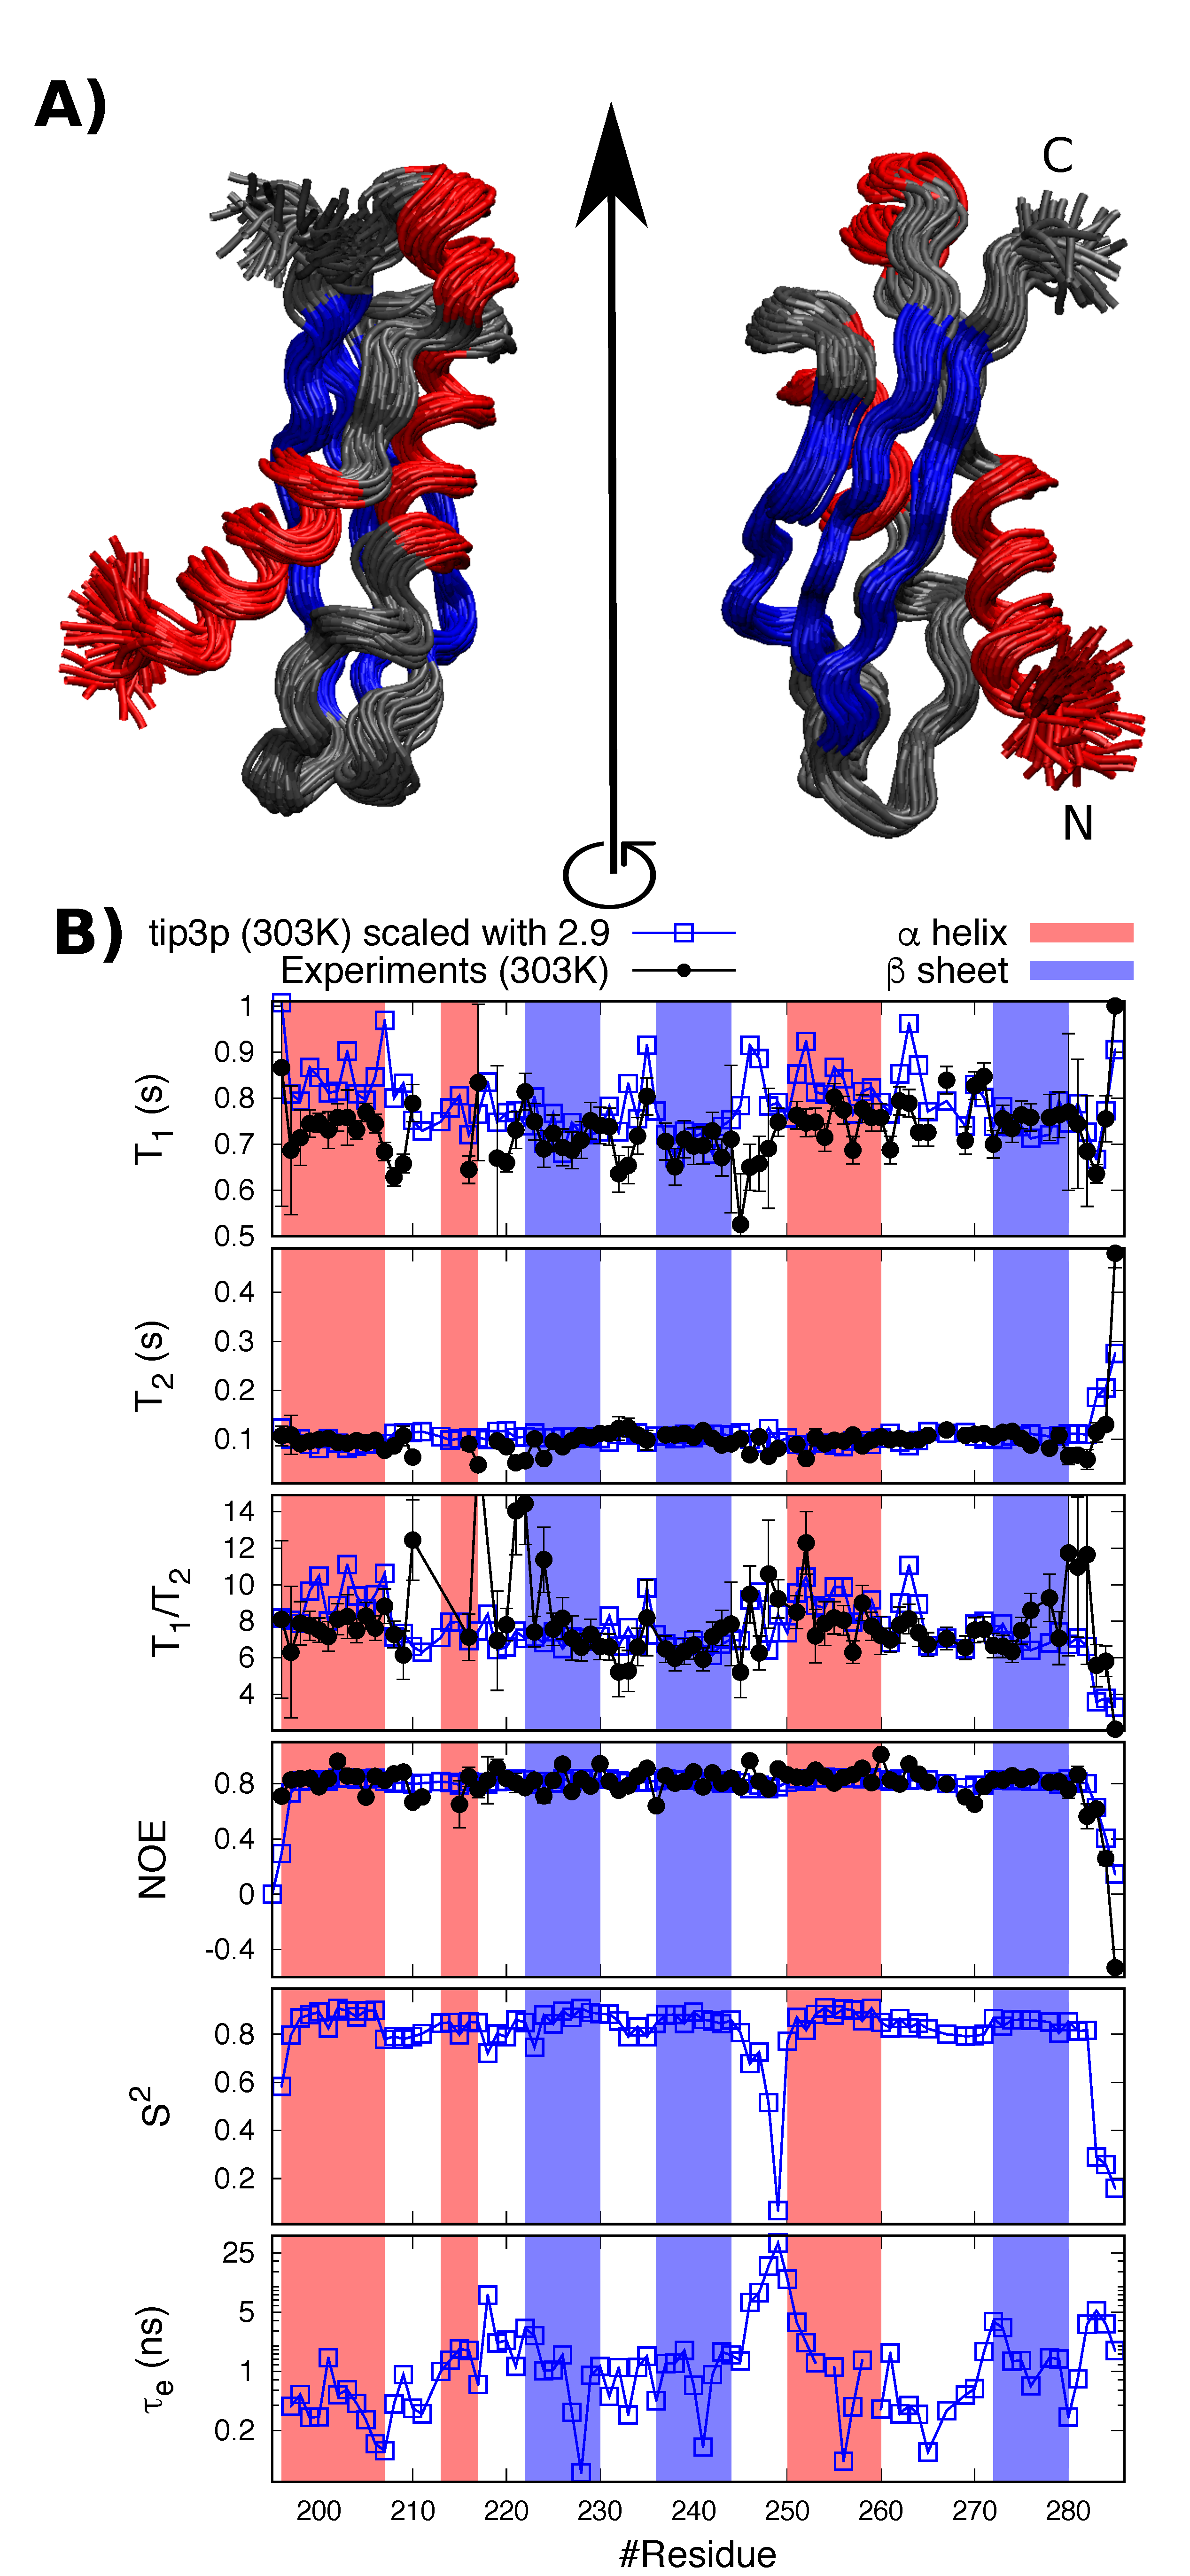
\includegraphics[width=8.5cm]{../Figs/RELdataHpTonB2.eps}%
  \caption{A) Structures sampled by HpTonB-92 from MD simulations with tip3p at 303~K
    (100 structures from 400ns long trajectory). Secondary structures
    are colour labelled with Visual Molecular dynamics \cite{frishman95,humphrey96};
    $\alpha$-helices are red and $\beta$-sheets are blue.
    B) Spin relaxation times from experiments and tip3p
    simulations with rotational diffusion coefficients divided by a
    constant factor of 2.9 at 303~K. Order parameters and effective internal correlation
    times calculated from simulations
    \label{HpTonBrelaxationDATAscaled}}%
\end{figure}

Simulations of PsTonB with tip4p or OPC4 water models,
shown in Fig. \ref{PsTonBrelaxationDATA}, give systemically
smaller $T_1$ values and $T_1/T_2$ ratio than experiments.
The effect of temperature difference of 12 degrees is significanlty
smaller than the different with experiments. Dividing the diffusion
coefficinents with a constant factor of 1.2 gives a good agreement for
spin relaxation rates between tip4p simulation and experiments at 298K,
as seen in Fig.~\ref{PsTonBrelaxationDATAscaled}.
\begin{figure}[!h]
  \includegraphics[width=8.5cm]{../Figs/PsTonBrelaxationDATA.eps}%
  \caption{Spin relaxation times for PsTonB from experiments \cite{??}
    and simulations with different water models. 
    \label{PsTonBrelaxationDATA}}%
\end{figure}
\begin{figure}[!h]
  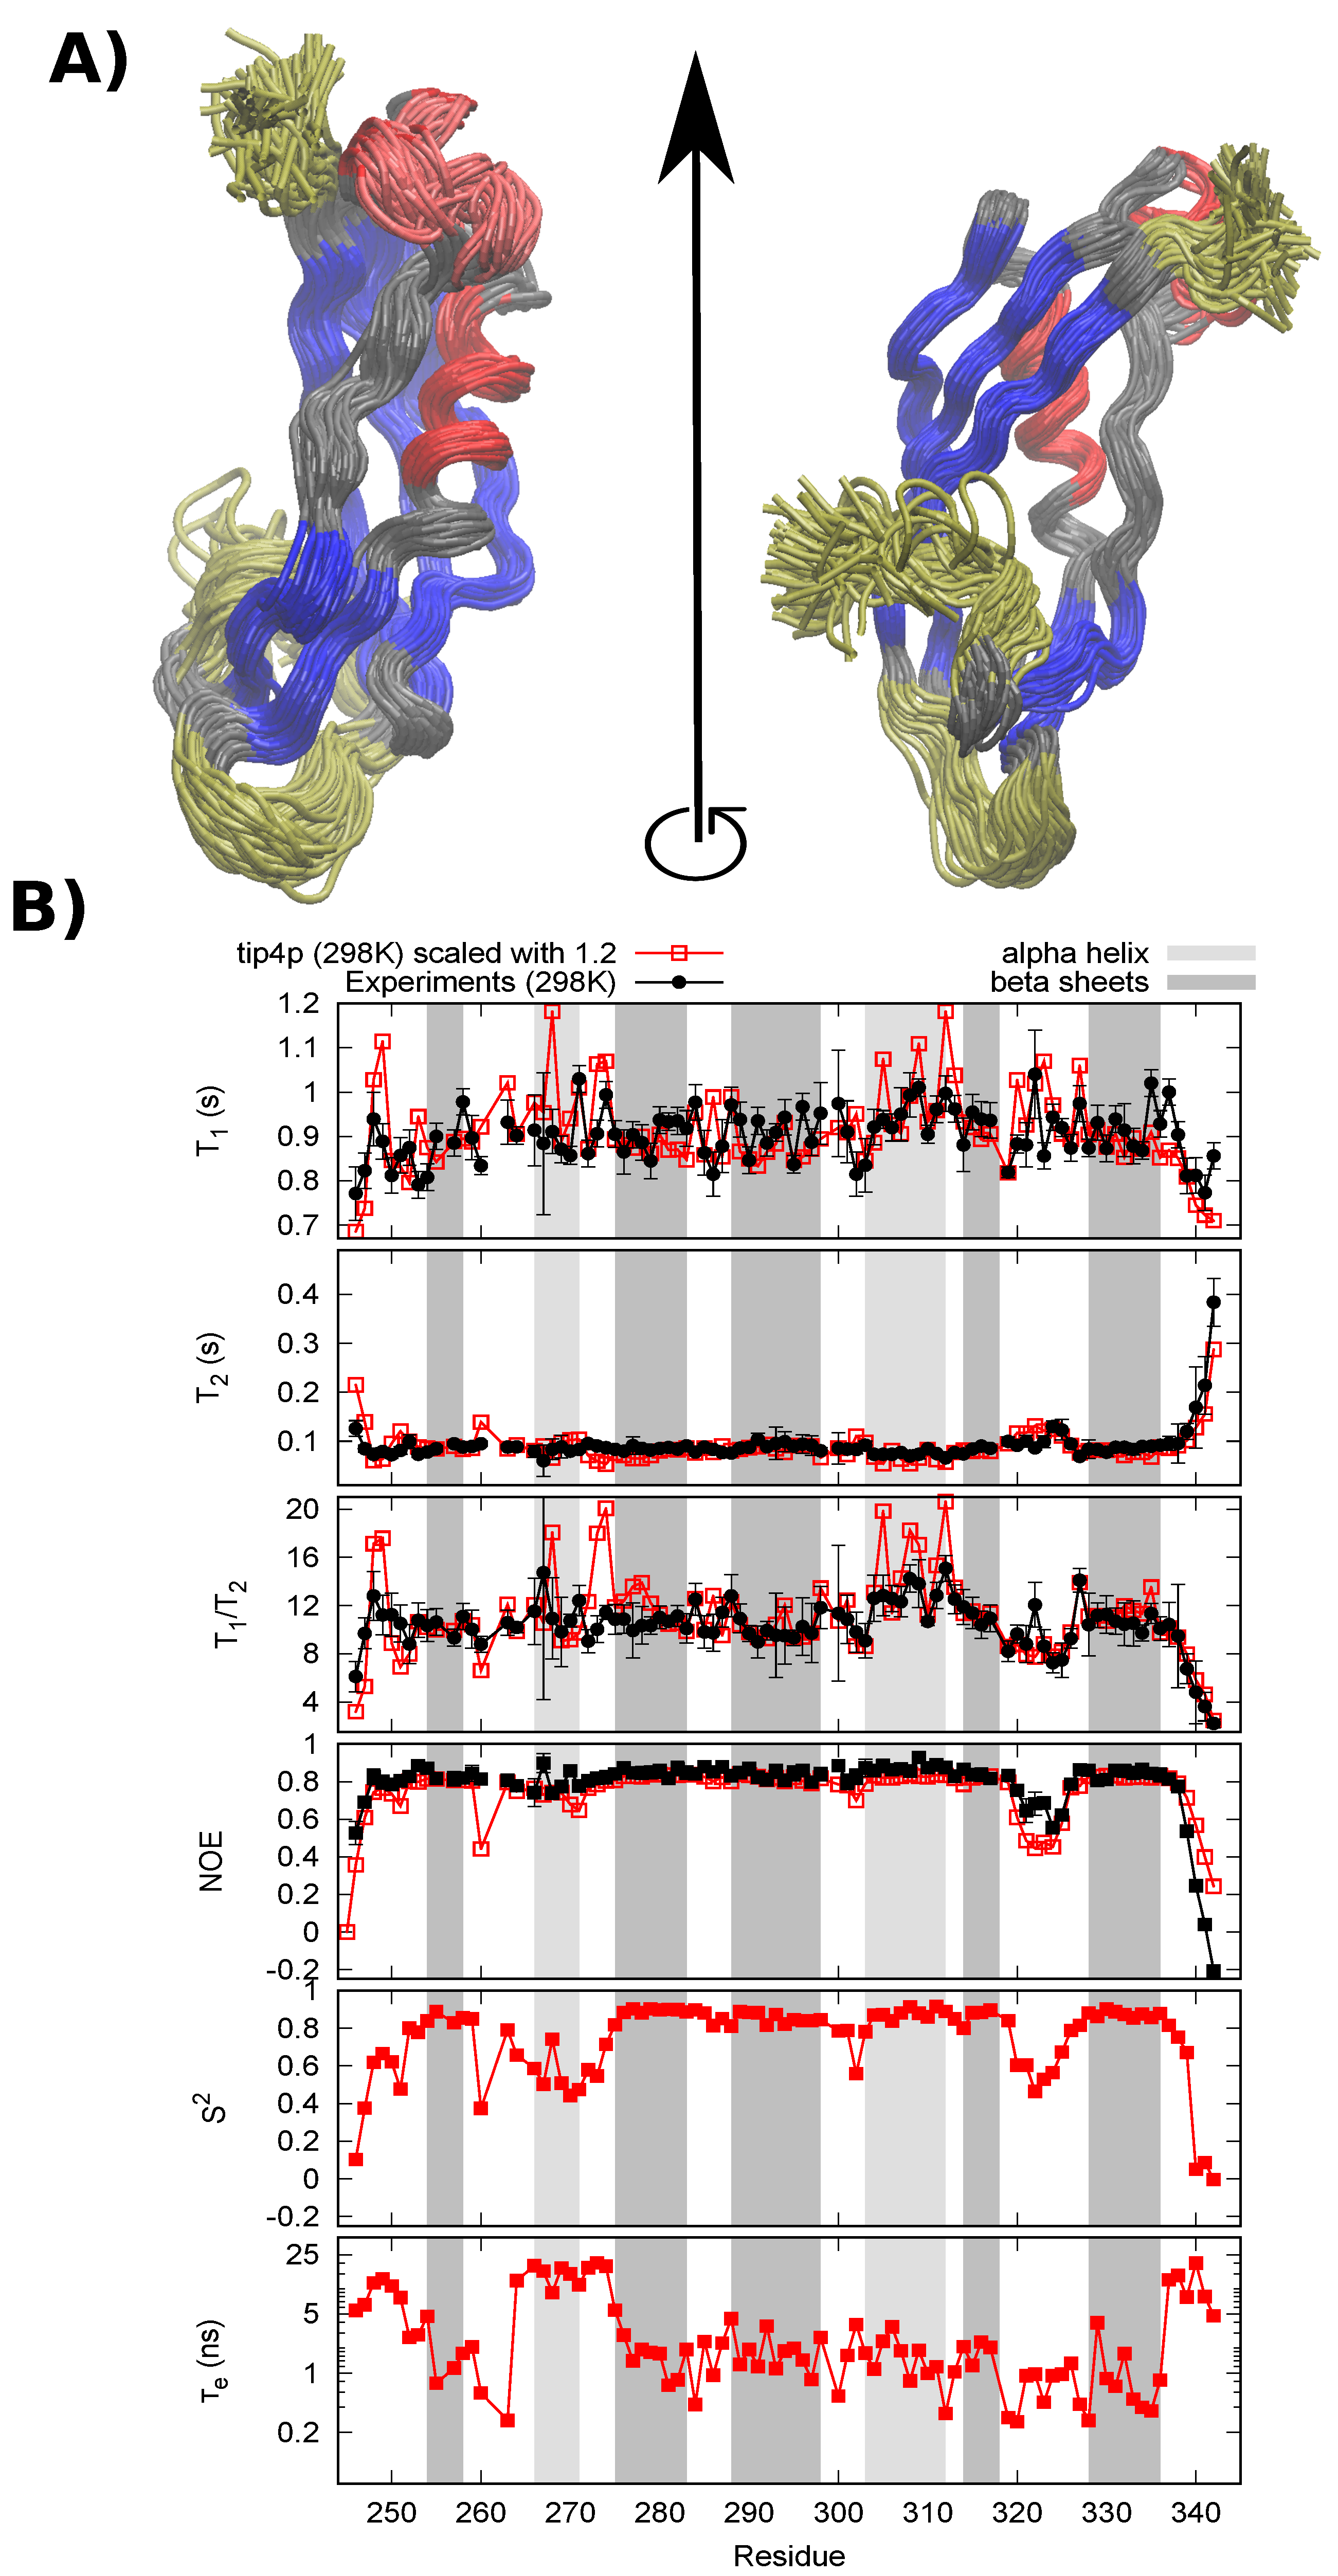
\includegraphics[width=8.5cm]{../Figs/RELdataPsTonB2.eps}%
  \caption{A) Structures sampled by PsTonB from MD simulations with tip4p at 298~K
    (100 structures from 400ns long trajectory). Secondary structures
    are colour labelled with Visual Molecular dynamics \cite{frishman95,humphrey96};
    $\alpha$-helixces are red and $\beta$-sheets are blue.
    Residues 246-251, 320-326 and 338-342 with increased internal dynamics are yellow and
    $\alpha$-helix sampling between two orientations (residues 266-270) is pink in the left column.
    B) Spin relaxation times from experiments and tip4p
    simulations with rotational diffusion coefficients divided by a
    constant factor of 1.2 at 298~K. Order parameters and effective internal correlation
    times calculated from simulations. \label{PsTonBrelaxationDATAscaled}}%
\end{figure}

The good agreement between spin relaxation data from experiments and
simulations with scaled diffusion coefficients suggests that the values
can be used to interpret the anisotropic diffusion of these proteins
from the measured NMR data. The scaled rotational diffusion coefficients
from MD models giving the best agreement with experimental spin relaxation
data are shown in Table \ref{ROTdiffCOEFFS}. The scaled diffusion coefficients
from tip3p simulations were chosen for HpTonB-92, because they give
slightly better overall agreement with experiments than simulations with
tip4p water model. The results are in line with values for more isotropic
proteins, which are previously determined by different methods to interpret
the spin relaxation data \cite{krishnan98}.
\begin{table}[!h]
  \centering
  \caption{Rotational diffusion coefficients scaled with constant factor which
    gives a good agreement for spin relaxation data,  2.9 for tip3p simulation of HpTonB
    and by 1.2 for tip4p simulation of PsTonB.}\label{ROTdiffCOEFFSscaled}
  \begin{tabular}{c c c c c}
    &    &  HpTonB-92  &  & PsTonB \\
    \hline
    D$_{xx}$    &   &   2.15 $\pm$ 0.01  & & 1.51  $\pm$ 0.01\\
    D$_{yy}$   &    &  2.43  $\pm$ 0.01  & & 1.72  $\pm$ 0.03\\
    D$_{zz}$   &    &  4.10   $\pm$ 0.01 & & 3.79  $\pm$ 0.03\\
    D$_{av}$  &    &   2.90  $\pm$ 0.03  & & 2.3  $\pm$ 0.02\\
    $\tau_{c}$(ns)  &    &  5.7   $\pm$ 0.1  & & 7.2 $\pm$ 0.1 \\
    %\hline
\end{tabular}
\end{table} 


%\begin{table}[htb]
%\centering
%\caption{Rotational diffusion coefficients (rad$^2\cdot 10^7$/s) calculated from HpTonB-92 simulations}\label{ROTdiffCOEFFShp}
%\begin{tabular}{c c c c c c c }
%            &  &  TIP3P  & &   TIP4P   &  &   OPC \\
%  \hline
%  D$_{xx}$   & &   0.083   & &   0.038   &  &   0.030 \\
%  D$_{yy}$   & &  0.077   &    &   0.033   &  &   0.027 \\
%  D$_{zz}$   & &  0.16    &    &   0.059   &  &    0.058 \\
%  2D$_{zz}$/(D$_{xx}$+D$_{yy}$) &  &   1.99    &  & 1.7    &	&  2.03 \\
%  D$_{av}$  &    &   0.11    &    &   0.043   &  &   0.038 \\
%  tau1     &  &  1.76	 &       &   4.13    &   &   4.87 \\
%  tau2     &  &  1.82	 &       &   4.40    &   &   5.14 \\
%  tau3     &  &  1.26	&        &   3.25    &   &   3.47 \\
%  tau4     &  &  1.05	 &       &    2.75   &   &  2.94 \\
%  tau5     &  &  3.05	 &       &    6.48   &   &   8.43 \\
  
  %\hline
%\end{tabular}
%\end{table} 

%Results with rotational diffusion coefficient corrected with constant factor
%are shown in Fig. \ref{relaxationDATAplotSCALED}. 
%\begin{figure}[!h]
%  \includegraphics[width=13cm]{/Users/osollila/Dropbox/TonB/Figs/relaxationDATAplotSCALED.eps}%
%  \includegraphics[width=13cm]{/home/samuli/Dropbox/TonB/Figs/relaxationDATAplotSCALED.eps}%
%  \caption{Relaxation parameters for HpTonB short construct from
%    experiments and simulations with Amber-ildn and different water models.
%    The rotational diffusion coefficients are divided by 3.0 for tip3p simulation
%    and by 1.3 for tip4p simulation.
%    Experiments are done in 303K and simulations in 310K, simulations in 303K are running.
%    \label{relaxationDATAplotSCALED}}%
%\end{figure}

%\begin{figure}[!h]
%  \includegraphics[width=13cm]{/Users/osollila/Dropbox/TonB/Figs/relaxationDATAplotLONGERconstructSCALED.eps}%
%  \includegraphics[width=13cm]{/home/samuli/Dropbox/TonB/Figs/relaxationDATAplotLONGERconstructSCALED.eps}%
%  \caption{PRELIMINARY RESULTS for relaxation parameters for HpTonB longer construct (107) from
%    experiments and simulations with Amber-ildn and tip4p water models.
%    The rotational diffusion coefficients are divided by 1.3.
%    Experiments and simulations are done in 303K.
%    \label{relaxationDATAplotSCALEDlongerCONSTRUCT}}%
%\end{figure}


%\begin{table}[htb]
%\centering
%\caption{Rotational diffusion coefficients scaled with constant factor which
%  gives a good agreement for spin relaxation data,  3.0 for tip3p simulation
%    and by 1.3 for tip4p simulation.
%  OPC RESULTS TO BE CHECKED.
%}\label{ROTdiffCOEFFS}
%\begin{tabular}{c c c c c c c }
%  rad$^2$/ns   &    &  TIP3P  &   &   TIP4P \\%  &  &   OPC \\
%  \hline
%  D$_{xx}$    &   &   0.028   &   &   0.029 \\%  &  &   0.030 \\
%  D$_{yy}$   &    &  0.026   &    &   0.025 \\%  &  &   0.027 \\
%  D$_{zz}$   &    &  0.053    &    &   0.045 \\%   &  &    0.058 \\
%  2D$_{zz}$/(D$_{xx}$+D$_{yy}$) &  &   1.99    &  & 1.7 \\%   &	&  2.03 \\
%  D$_{av}$  &    &   0.034    &    &   0.033 \\%  &  &   0.038 \\
  %\hline
%\end{tabular}
%\end{table} 



\subsection{Interpretation of protein internal relaxation from MD simulations}
Experimental spin relaxation times are well reproduced by MD simulation
data when overall rotational diffusion is scaled with a constant factor,
as seen in Figs. \ref{HpTonBrelaxationDATAscaled} and \ref{PsTonBrelaxationDATAscaled}.
Thus, the simulations can be used to interpret internal relaxation processes
observed in spin relaxation experiments for proteins.

NMR experiments and the most realistic MD simulation
based model show very little variation between spin relaxation times for
different residues in HpTonB-92 as seen in Fig. \ref{HpTonBrelaxationDATA}.
This indicates a rigid protein structure, which is also seen in
MD simulation snapshots overlayed in Fig. \ref{HpTonBrelaxationDATA} A).
Enhanced conformational sampling is seen only for few residues in terminal
ends, which are also visible in spin relaxation data.
Some deviation from average spin relaxation times are observed also
between residues 210-222, which probably arises from sampling between
two orientations of the $\alpha$-helix (see discussion below and in Ref. \cite{??}).
Exceptionally low order parameters and long effetive correlation times
are also observed for residues 245-250 in simulations and the same region
gives small $T_1$ times in experiments. However, the interpretation of
these observations is not straightforward, because low $T_1$ in this region
are not reproduced by simulations. More detailed discussion together with
longer HpTonB construct is presented elsewhere \cite{??}.

More variety in internal dynamics between residues is found for PsTonB protein,
as seen in Fig. \ref{PsTonBrelaxationDATAscaled}. Segments
with enhanced conformational sampling are labelled with yellow colour
in Fig. \ref{PsTonBrelaxationDATAscaled} A).
The terminal ends show significantly enhanced conformational sampling
in MD simulation snapshots, which is also observed in spin relaxation times
from simulations and experiments. The terminal ends are also characterized
by low order parameters and long effective internal correlation times
arising from larger amount of sampled conformational states.
Enhanced conformational sampling is also observed for residues between 320-326,
which is a loop between two $\beta$-sheets.
Low order parameters and long internal effective correlation times are also
observed in MD simulations for residues between 260-274, which similar region
as residues 210-222 in HpTonB-92. In this case the simulations reveal
two different orientations sampled by the $\alpha$-helix in this region
(colour labelled with pink in Fig.~\ref{PsTonBrelaxationDATA} A)), which
also explains the lower resolution in NMR spectra for this region
observed for PsTonB and HpTonB constructs \cite{??}.
%In addition to Spin relaxation rate deviations from baseline
%are observed for residues 246-251 in N-terminus,
%and residues 338-342 in C-terminus.
%Also order parameters are low and effective internal
%relaxation times long for these segements as seen in Fig. \ref{??} B).
%In addition, low order parameters and larger effective correlation times
%are observed for PsTonB residues 260-274 and 300-303
%in Fig. \ref{PsTonBrelaxationDATA} B).
%Low order parameters and large
%effective correlation times between residues 300-303 are not seen
%in spin relaxation data, thus it is not clear if these arise from
%simulation artefact.

Relaxation processes can be further quantified by analysing the timescales,
which lead to spin relaxation times in agreement with experiments.
This is exemplified in Fig. \ref{coeffsPLOT} by plotting the prefactors corresponding
each timescale after fitting Eq. \ref{gprime_fit} to MD simulation data. 
The same residues for PsTonB as in Fig. \ref{exampleCORRF} are used.
Rotational relaxation of residue 331 in $\beta$-sheet is dominated
by timescales of $\sim$5.5~ns and $\sim$8~ns, which arise from global rotation
of protein. Only a small fraction of relaxation arises from fast internal motions,
as expected for rigid structure with large order parameter value. Rotational
relaxation of residue 322 in flexible loop is also dominated by timescales
around $\sim$8~ns corresponding overall rotational diffusion, but fast motions
related to internal protein dynamics are more significant than for the $\beta$-sheet
residue in agreement with lower order parameter value. On the other hand,
rotational dynamics of residue 341 in N-terminal is dominated by timescales
below 3~ns related to the internal protein relaxation. The contribution from timescales
close to $\sim$13~ns is probably related to slow conformational sampling of
N-terminus, rather than overall rotational dynamics. This is in agreement with
Fig. \ref{PsTonBrelaxationDATA}, suggesting that sampling of large amount of
conformations leads to small order parameters and large effective correlation times.
\begin{figure}[!h]
  
\includegraphics[width=8.5cm]{../Figs/coeffsPLOT.eps}%
  \caption{Prefactors $A_i$ corresponding different timescales $\tau_i$ in Eq.\ref{gprime_fit}
    from correlation functions giving a good agreement with experimental spin relaxation times
    for PsTonB at 298K. 
    \label{coeffsPLOT}}%
\end{figure}



\section{Discussion and conclusions}
Protein rotational dynamics was separated to the overall
brownian tumbling around protein intertia axes and internal
conformational sampling. The overall rotational diffusion constants
were calculated from the slope of mean square angle deviations (Eq. \ref{DIFFdef}),
which were found to be essentially linear for all inertia axes.
The results indicate that monomeric proteins in dilute solution
experience rotational brownian tumbling in agreement with previous
MD simulation study \cite{wong08}. Only a small subdiffusive behaviour
was found with short timescales below 0.12 ns. This result can be used as a constrast
for crowded environment, where anomalous diffusion is expected to
be more significant \cite{hofling13}.

General form of rotational correlation function for anisotropic rigid body
(Eq.~\ref{CORRFanisot}) with timescales from rotational diffusion constants
was successfully fit to the overall rotational correlation functions from
MD simulations for all individual N-H bonds. Furthermore, the new correlation
functions calculated from Eq.~\ref{newCORRF} were in good agreement with
the total correlation functions calculated from original trajectories.
The results suggest that the intertia axes can be used to describe
the overall rotational diffusion as a good approximation and that
the assumption of separation of internal and overall rotational
relaxation (Eq.~\ref{??}) is a good approximation for the studied
proteins, as observed previously also for other protein~\cite{wong08,allner15}.

Using the new correlation functions from Eq.~\ref{newCORRF} in
spin relaxation time calculations reduces the statistical fluctuations
arising from longer lag times in correlation function calculation,
which allows the higher accuracy with less simulation data.
The essential reason is that the rotational diffusion constants
can be determined by fitting a single parameter (linear slope) which is
more robust than fitting exponential function with several parameters to
a correlation function calculated from MD simulation. After determining
the diffusion constants and using Eq.~\ref{newCORRF} the overall
part of correlation functions do not have statistical fluctuations
in spin relaxation time calculations.

Comparison to experimental results revealed that overall rotational diffusion
coefficients were overestimated by a factor of $\sim$3 in simulations with tip3p
water, in agreement with previous studies \cite{prompers02,wong08,anderson12}. Simulations
with tip4p and opc4 water models gave more realistic diffusion coefficients,
which overestimated diffusion only with factors $\sim$1-1.2.
The realistic overall rotational dynamics was determined by
scaling the diffusion coefficients to all directions post-simulationally by the
same constant factors such that the calculated $T_1/T_2$ was in optimal
agreement with experiments. Similar correction has been done previously
for proteins with isotropic rotational diffusion with single exponential rotational correlation
function \cite{showalter07a,showalter07b,maragakis08,gu14,allner15}.
Alternatively only order parameters are used in the comparison with
experiments~\cite{gu14,maragakis08,trbovic08,best04}.
Overall rotational diffusion is previously corrected for anisotropic
molecules by using isotropic reorientational eigenmode dynamics (iRED)~\cite{prompers02}
or quaternions~\cite{anderson12}. The advantage of these approaches is that
the separation between internal and overall rotational dynamics is not
required, thus they would be applicable also for intrinsically disoredered
proteins. However, the correction of overall rotational diffusion is based on
the assumption that incorrect diffusion arises from incorrect water viscosity.
Thus, a model with correct overall rotational diffusion is required to
compare intrinsically disordered molecule simulations to experimental
relaxation data.

%or correcting overall rotation by using quaternions \cite{anderson12} or
%fitting timescales to satisfy experiments \cite{prompers02} or
%These approaches are not, however, useful for anitropic proteins and order
%parameter comparison is not direct comparison between simulations and experiments in
%the case of freely rotating molecules. 

%, which resulted scaling factor of 1.2 for
%PsTonB simulation with tip4p and factor 2.9 for HpTonB with tip3p.
%The overstimated overall diffusion
%coefficient can be corrected post-simulationally to compare internal dynamics
%and order with experiments. 
%As already observed previously
%In addition, diffusion constants can be scaled with a constant
%factor before calculating the new correlation functions to compensate
%the overestimated rotational diffusion due to inaccuracies in some
%water models.

A good agreement between spin relaxation times from experiments and simulations is
found after overall rotational diffusion constants are scaled with a constant
factor. This allows the interpretation of internal protein dynamics
from spin relaxation times by using MD simulations even with tip3p water model.
Here we use the approach to indentify dynamical regions in two proteins,
HpTonB-92 and PsTonB with relatively rigid structures. However, the
approach could be useful for intepretation of spin relaxation data from
proteins with more regions containing complicated local dynamics, like
Calmodulin~\cite{trjandra95}.


% If you have acknowledgments, this puts in the proper section head.
\begin{acknowledgments}
% Put your acknowledgments here.
  %OHSO acknowledges Aalto science IT project and
  We acknowledge CSC-IT center for science for computational resources %, and Emil Aaltonen foundation for funding.
\end{acknowledgments}

% Create the reference section using BibTe
\bibliography{refs.bib}

%\newpage
%\appendix
\begin{center}
{\bf SUPPLEMENTARY INFORMATION}
\end{center}
\begin{figure*}[!h]
  \includegraphics[width=16.5cm]{../Figs/RMASDplotPsTonBtip4pT310K.eps}%
  \caption{The intertia tensor angles as a function of time and mean square angular
    deviations for PsTonB simulation with tip4p water model at 310K.
    \label{RMASDplotLOG310}}%
\end{figure*}
\begin{figure*}[!h]
  \includegraphics[width=16.5cm]{../Figs/RMASDplotPsTonBtip4pT298K.eps}%                                                                                                    
  \caption{The intertia tensor angles as a function of time and mean square angular
    deviations for PsTonB simulation with tip4p water model at 298K.
    \label{RMASDplotLOG298}}%                                                                                                                                                  
\end{figure*}


%\todolist
\end{document}
%
% ****** End of file aiptemplate.tex ******
